% \documentclass[xelatex,xcolor={dvipsnames}]{beamer}
\usepackage{times}
%\usepackage[utf8x]{inputenc}
% \usepackage[T1]{fontenc}
% \usepackage{mathptmx}  
 \usepackage{fontspec} % xltxtra
 \defaultfontfeatures{Ligatures=TeX}
%	\setmainfont[Renderer=ICU]{Charis SIL}
%	\setmainfont[Renderer=ICU]{Brill}
	\setmainfont[Renderer=ICU]{Libertinus Serif}
%	\setmainfont[Renderer=ICU]{Libertinus Sans}
	\usefonttheme{serif}
 %	\newfontfamily{\H}[Scale=1,Script=Hebrew]{David CLM} %{Frank Ruehl CLM}%{Ezra SIL}
\usepackage{colortbl,multirow,amsmath,amssymb,url,natbib,graphicx}
%\usepackage[dvipsnames]{xcolor}
%\usepackage{graphicx,colortbl,multirow,amsmath,amssymb,url} %natbib
\usepackage{pbox}
\usepackage{pifont}
%\usepackage{hyperref}
% \usepackage{geometry,vmargin,setspace,lscape} %rotating
\usepackage{xytree}
\usepackage{stmaryrd,wasysym}
\usepackage{arydshln}
\usepackage{array} %tabular column formatting
\usepackage{dashrule} %\hdashrule
\usepackage{siunitx} %decimals in tables

\bibpunct[:]{(}{)}{;}{a}{}{,} %\usepackage{dashrule}
		\setlength{\bibsep}{0pt plus 0.3ex}
\usepackage[normalem]{ulem}
\providecommand{\tightlist}{%
	\setlength{\itemsep}{0pt}\setlength{\parskip}{0pt}}

\usepackage{tipa}
\usepackage{expex}
	\lingset{aboveexskip=0.1ex,belowexskip=0.1ex,aboveglftskip=-0.1ex,interpartskip=0.1em,labelwidth=!6pt,belowpreambleskip=0.1ex} %, *=*?}
	\resetcountonoverlays{excnt}
\newcommand\trace{\rule[-0.5ex]{0.5cm}{.4pt}}
\usepackage[nocenter]{qtree}
\usepackage{tikz}
	\tikzstyle{every picture}+=[remember picture]

\newenvironment{dummy}{}{}
% \AtBeginSection[]{}
% \setbeameroption{show notes on second screen}
% \setbeameroption{show notes}

% \usetikzlibrary{shapes.geometric, arrows}
% \newlength{\bls}
% \setlength{\bls}{\baselineskip-\doublerulesep+1pt} % for double cline, uses package calc
% \newcommand\ipa[1]{\textipa{#1}}
\let\it\textit
\newcommand\zero{\O{}}
\newcommand\gsc[1]{\textsc{\lowercase{#1}}} %for glossing in small caps - comment out to return to caps
\newcommand\citey[1]{{\scriptsize #1}}
  \renewcommand\root[1]{$\sqrt{\text{\gsc{#1}}}$}
\newcommand{\cmark}{\ding{51}}% 52
\newcommand{\xmark}{\ding{55}}%
 \newcommand{\hand}{\ding{43}}

% \newcommand\hammer[1]{\begin{center}\fbox{\parbox{0.9\linewidth}{\centering \textsf{#1}}}\end{center}}
% \newcommand\hammersmall[1]{\begin{center}\fbox{\parbox{0.3\linewidth}{\centering \textsf{#1}}}\end{center}}
\newcommand\blue[1]{\textcolor{blue}{#1}} \newcommand\red[1]{\textcolor{red}{#1}}
% \newcommand\green[1]{\textcolor{ForestGreen}{#1}}
\newcommand\olive[1]{\textcolor{olive}{#1}}
 \newcommand\gray[1]{\textcolor{gray}{#1}}
\newcommand\denote[1]{$\llbracket$#1$\rrbracket$}

\newcommand\lra{$\leftrightarrow$}
\newcommand\dgs[1]{\textsubarch{#1}}
	\newcommand\vz{\text{Voice$_{\text{[--D]}}$}}
	\newcommand\vd{\text{Voice$_{\text{[+D]}}$}}
	\newcommand\pz{\text{$p_{\text{[--D]}}$}}
	\newcommand\va{\root{\gsc{ACTION}}}
	\newcommand{\tkal}{\emph{XaYaZ}}
	\newcommand{\tpie}{\emph{Xi\dgs{Y}eZ}}
	\newcommand{\tpua}{\emph{Xu\dgs{Y}aZ}}
	\newcommand{\mpua}{\emph{meXu\dgs{Y}aZ}}
	\newcommand{\thif}{\emph{heXYiZ}}
	\newcommand{\thuf}{\emph{huXYaZ}}
	\newcommand{\mhuf}{\emph{muXYaZ}}
	\newcommand{\thit}{\emph{hitXa\dgs{Y}eZ}}
	\newcommand{\tnif}{\emph{niXYaZ}}
\newcommand\del[1]{$<$#1$>$}

%=== shortcuts for ROOT  types ========== % 

%  explicit creation roots: <s, t> 
% (the s here is s_e), and the type of all our vPs
% we will have subscript versions of each type too
\newcommand{\set}{${{\langle}s_{e}, t{\rangle}}$} 
\newcommand{\setsub}{$_{{\langle}s_{e}, t{\rangle}}$}  % because I can't get these subscripted 

%  implicit creation roots: <e, t> 
\newcommand{\et}{${{\langle}e, t{\rangle}}$} 
\newcommand{\etsub}{$_{{{\langle}e, t{\rangle}}}$} % for subscripting

%  <e, <s_s, t>> for change of state roots 
\newcommand{\esst}{${\langle}e, {\langle} s_{s}, t{\rangle}{\rangle}$} 
\newcommand{\esstsub}{$_{{\langle}e, {\langle} s_{s}, t{\rangle}{\rangle}}$} 

\newcommand{\estsub}{$_{{\langle}e, {\langle} s, t{\rangle}{\rangle}}$} 

\newcolumntype{a}{>{\columncolor{red}}c}
\newcolumntype{b}{>{\columncolor{cyan}}c}
\newenvironment{rcases}
  {\left.\begin{aligned}}
  {\end{aligned}\right\rbrace}
%\tikzstyle{input} = [draw, inner sep=0.4cm, outer sep=0, minimum width=2cm, text height=1.6cm, align=center, text centered, draw=black, fill=blue!30]
%\tikzstyle{root} = [ellipse, minimum height=1cm, text width=1cm, align=center, text centered, draw=black, fill=green!30]
%\tikzstyle{lexeme} = [draw, inner sep=0.1cm, outer sep=0, text width=1.3cm, text height=0.2cm, align=center, text centered, draw=black, fill=orange!30, node distance=1.7cm]
%\tikzstyle{template} = [rectangle, rounded corners, minimum width=1.3cm, minimum height=1cm, text centered, draw=black, fill=red!30]
%\tikzstyle{label} = [font=\scshape]
%\tikzstyle{arrow} = [thick, ->, >=latex]
%\tikzstyle{relate} = [dotted, thick]

% \makeatletter %Allow superscript ^ and subscript _
% \catcode`_=\active%
% \gdef_#1{\ensuremath{{}\sb{#1}}}%
% \catcode`^=\active%
% \gdef^#1{\ensuremath{{}\sp{#1}}}%
% \makeatother

\setbeamercovered{transparent}
\usecolortheme[RGB={0,50,95}]{structure}
\setbeamercolor{alerted text}{fg=red}

\usepackage{etoolbox}
\makeatletter
\preto{\appendix}{%
	\patchcmd{\beamer@continueautobreak}{\refstepcounter{framenumber}}{}{}{}}
\makeatother

\setbeamertemplate{blocks}[rounded][shadow=true]
\setbeamertemplate{navigation symbols}{}
%\useoutertheme{infolines}
%\setbeamertemplate{frametitle}[default][center] 

%\usepackage{beamerthemeshadow}
\usetheme{Madrid}

\let\expexgla\gla % conflict with unicode-math package, which pandoc/beamer autoloads
\AtBeginDocument{\let\gla\expexgla}

\title{Lexical processing}
\author{Itamar Kastner}
%institute{}
\date{Morphology, UoE 2023-24}

%\setbeamertemplate{blocks}[rounded][shadow=true]
%\setbeamertemplate{navigation symbols}{}
\useoutertheme{infolines}
%\setbeamertemplate{frametitle}[default][center] 
%\usetheme{Madrid}

\begin{document}


\frame{\titlepage}


\frame{\frametitle{Goals}
\begin{itemize}
	\item Discuss	 one major	 issue of	 morphology	 in	 the	  psycholinguistic	 and neurolinguistic	literature.	
	  
	\item Most studies	 ask	 whether	 words	 decompose	 into	morphemes	 during	 language	 recognition	 and	 production.
	  
	\item Some	 hypotheses	 suggest	 that	 decomposition	 varies	  depending	 on	 the	 ``transparency'' or	 ``regularity'' of	 the	morphology.
  
	\item   We'll	 look	 at	 evidence	 that	 words	 are	  decomposed	 no	 matter	 how	 ``opaque'' and	 ``irregular''.
    
%    \item And at the role of experience and frequency.
\end{itemize}
}

\frame{\frametitle{Words or Morphemes}
\begin{block}{Decomposition vs storage}
	\begin{itemize}
		\item \alert{\textbf{Storage:}} we store whole stems.
		\item \alert{\textbf{Decomposition:}} we store smaller elements (morphemes) and decompose the input.
		\item A lot of work has been devoted to finding out where the line should be drawn. 
	\end{itemize}
\end{block}
}


\frame{\frametitle{Experimental Paradigms}
\begin{block}{\alert<1>{\textbf{Lexical decision}}}
	\begin{itemize} \tightlist
		\item Response Time $\sim$ frequency + other stuff.
		\item Error rate (Accuracy) $\sim$ + other stuff.
		\item The most robust measure we have.
		% \item Though we still don't understand it completely:
			\begin{itemize}
			\item What's the computation? Need a theory of the task.
			\item For morphology, is it about lookup? Combination of stem and affix?
			\item Do we need a theory of storage or of retrieval?
			\end{itemize}
	\end{itemize}
\end{block}

\begin{block}{\alert<2>{\textbf{Priming}}}
	\begin{itemize} \tightlist
		\item Prime and target.
		\item Masked priming.
		\item Identity prime.
		\item Semantic prime.
		\item Form prime?
	\end{itemize}
\end{block}
}

	\subsection{Affix stripping}
\frame{\frametitle{\insertsubsection{}: \cite{taft79}}
	\begin{center}
	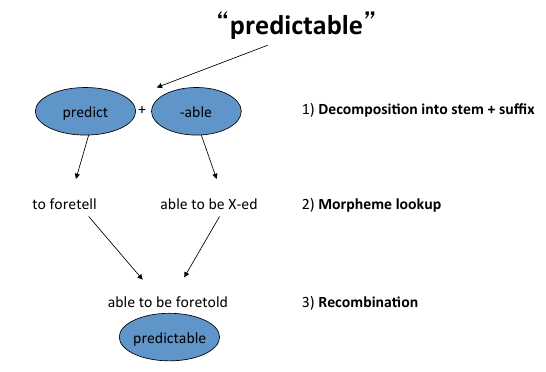
\includegraphics[width=0.75\textwidth]{figs/taft.png}
	\end{center}
	
	Decomposition, lookup and recombination can be affected by:
		\begin{itemize} \tightlist
			\item \alert<2>{\textbf{Surface}} frequency.
			\item \alert<2>{\textbf{Base}} frequency.
		\end{itemize}

}


\frame{\frametitle{Priming Predictions}
Does \emph{nation} prime \emph{national}?

\pause

	\begin{block}{Storage}
	\begin{itemize} \tightlist
		\item \alert<2>{\textbf{Yes!}}
			\begin{itemize} \tightlist
				\item Similar phonology.
				\item Similar semantics.
			\end{itemize}
	\end{itemize}
	\end{block}

\pause
	
	\begin{block}{Decomposition}
	\begin{itemize} \tightlist
		\item \alert<3>{\textbf{Yes!}}
			\begin{itemize} \tightlist
				\item Decompose \emph{national} to \emph{nation}+\emph{al}.
				\item Identity priming for \emph{nation}.
			\end{itemize}
	\end{itemize}
	\end{block}
}


	\subsection{Behavioral findings}

\frame{\frametitle{\insertsubsection: \cite{rastleetal00}}

	How can we disentangle semantics, phonology and form?

	\begin{block}{Methods and results}
		\begin{columns}[t]
			\begin{column}{0.65\textwidth} \small
				\vspace{-9em}
				
				\begin{itemize} \tightlist
					\item Masked priming.
					\item SOAs: 43ms, 73ms, 230ms.
				\end{itemize}

				\begin{tabular}{lll@{ --- }l}
					\cmark & \alert<1>{\textbf{Identity:}} & church & CHURCH\\
					\cmark & \alert<1>{\textbf{Morpho + Sem + Form:}} & adapt\blue{er} & ADAPT\blue{ABLE}\\\hdashline
					\xmark & Sem + Form: & screech & SCREAM\\
					\xmark & Sem: & cello & VIOLIN\\
					\xmark & Form: & typhoid & TYPHOON\\
				\end{tabular}
			\end{column}
			\begin{column}{0.3\textwidth}
				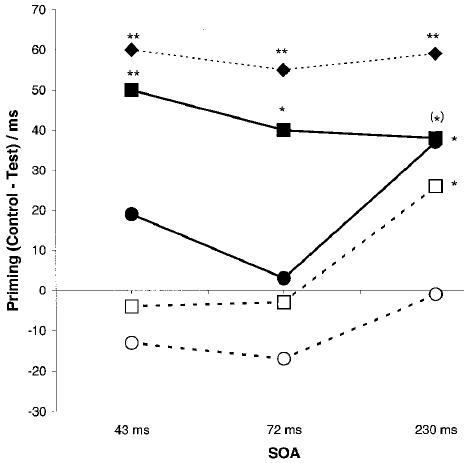
\includegraphics[width=1\textwidth]{figs/rastle2.png}
			\end{column}
		\end{columns}
	\end{block}

\pause

	\begin{itemize} \tightlist
		\item Stimuli are \alert<2>{\textbf{obligatorily}} (automatically) decomposed into stem and affix.
		\item Morpho $\approx$ Identity.
		\item Morpho $\ne$ Form + Meaning (phonesthemes).
	\end{itemize}

	\ding{228} What about things that only look like affixes?

}


%\frame{\frametitle{\insertsubsection: \cite{rastleetal00}}
%	\begin{block}{Conditions}
%		\begin{tabular}{lll@{ --- }l}
%			\cmark & \textbf{Identity:} & church & CHURCH\\
%			\cmark & \textbf{Morpho + Sem + Form:} & adapt\blue{er} & ADAPT\blue{ABLE}\\\hdashline
%			\xmark & \textbf{Meaning + Form:} & screech & SCREAM\\
%			\xmark & \textbf{Meaning:} & cello & VIOLIN\\
%			\xmark & \textbf{Form:} & typhoid & TYPHOON\\
%		\end{tabular}
%	\end{block}
%	
%	\begin{block}{Method}
%		\begin{itemize} \tightlist
%			\item Masked priming.
%			\item SOAs:
%				\begin{itemize} \tightlist
%					\item 43ms
%					\item 73ms
%					\item 230ms
%				\end{itemize}
%		\end{itemize}
%	\end{block}
%}
%
%\frame{\frametitle{\insertsubsection: \cite{rastleetal00}}
%	\begin{center}
%		\includegraphics[width=0.8\textwidth]{figs/rastle1.png}
%	\end{center}
%	
%	\begin{itemize} \tightlist
%		\item Morpho $\approx$ Identity.
%		\item Morpho $\ne$ Form + Meaning (phonesthemes).
%	\end{itemize}
%}


\frame{\frametitle{\insertsubsection: \cite{rastleetal04}}
	\begin{block}{Obligatory decomposition}
		\begin{tabular}{lll@{ --- }l}
			\cmark & \alert<1>{\textbf{Semantic:}} & \emph{clean\blue{er}} & CLEAN\\
			\cmark & \alert<1>{\textbf{Psuedo-morphological:}} & \emph{corn\blue{er}} & CORN \\\hdashline
			\xmark & Form: & \emph{broth\green{el}} & BROTH
		\end{tabular}
	\end{block}
		
	\begin{itemize} \tightlist
		\item \emph{broth\blue{er}} primes BROTH.
		\item \emph{broth\green{el}} does not prime BROTH.
		\item Readers identify the \alert<1>{\textbf{visual form}} of the suffix -\blue{er}.
	\end{itemize}
	
	\bigskip
	
	\ding{228} How far can we stretch this? What about \alert<2>{\textbf{irregular morphology}}?
}

%\frame{\frametitle{The Past Tense Debate}
%	\begin{block}{Word and rules?}
%		\begin{itemize} \tightlist
%			\item The \alert<1>{\textbf{storage}} model (Pinker):
%				\begin{itemize} \tightlist
%					\item Rules for regular verbs.
%					\item Storage for irregular verbs.
%				\end{itemize}
%			\item The \alert<2>{\textbf{decomposition}} model:\\
%					\only<2>{
\includegraphics[scale=0.4]{figs/decomposeall.jpg}}
%		\end{itemize}
%	\end{block}
%}


\frame{\frametitle{\insertsubsection: Priming for Irregulars?} \small
	\begin{block}{No: Marslen-Wilson et al (1993)}
		\begin{itemize} \tightlist
			\item Cross-modal priming: \emph{taught} does not prime TEACH.\\
			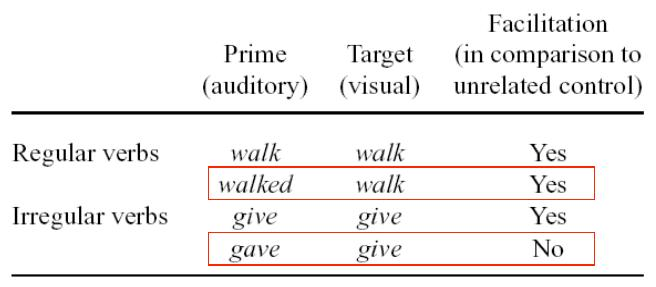
\includegraphics[scale=0.23]{figs/marslen93.jpg}
		\end{itemize}
	\end{block}
%\pause
	\begin{block}{Yes: Marslen-Wilson and Tyler (1998)}
		\begin{itemize} \tightlist
			\item Long-lag priming: \emph{taught} does prime TEACH.\\
			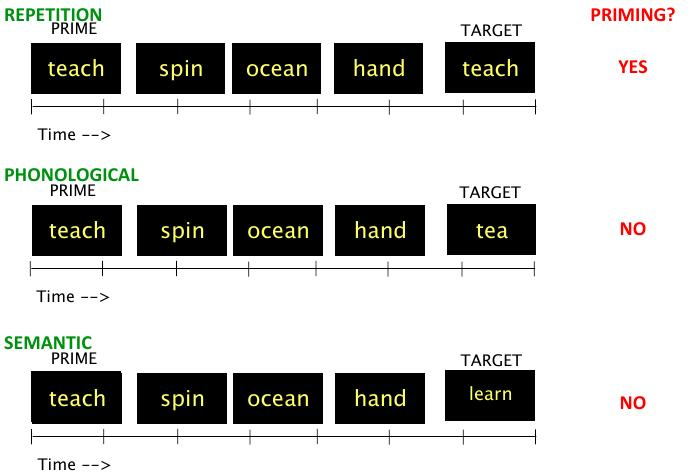
\includegraphics[height=0.35\textheight]{figs/marslen98.jpg}
				\hfill
				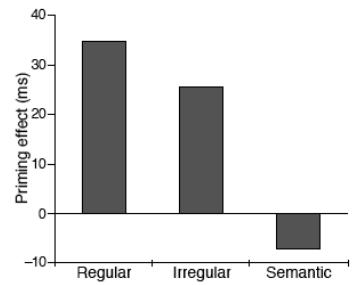
\includegraphics[height=0.35\textheight]{figs/marslen98b.jpg}
			
		\end{itemize}
	\end{block}
}

\frame{\frametitle{Interim Summary}
	\begin{enumerate}
		\item Suffixed nouns and adjectives are decomposed.
		\item Decomposition is obligatory.
		\item Unclear from behavioral methods whether irregular verbs are decomposed.
	\end{enumerate}
}


	\subsection{MEG background}
\frame{\frametitle{\insertsubsection}
    \only<1>{\begin{center}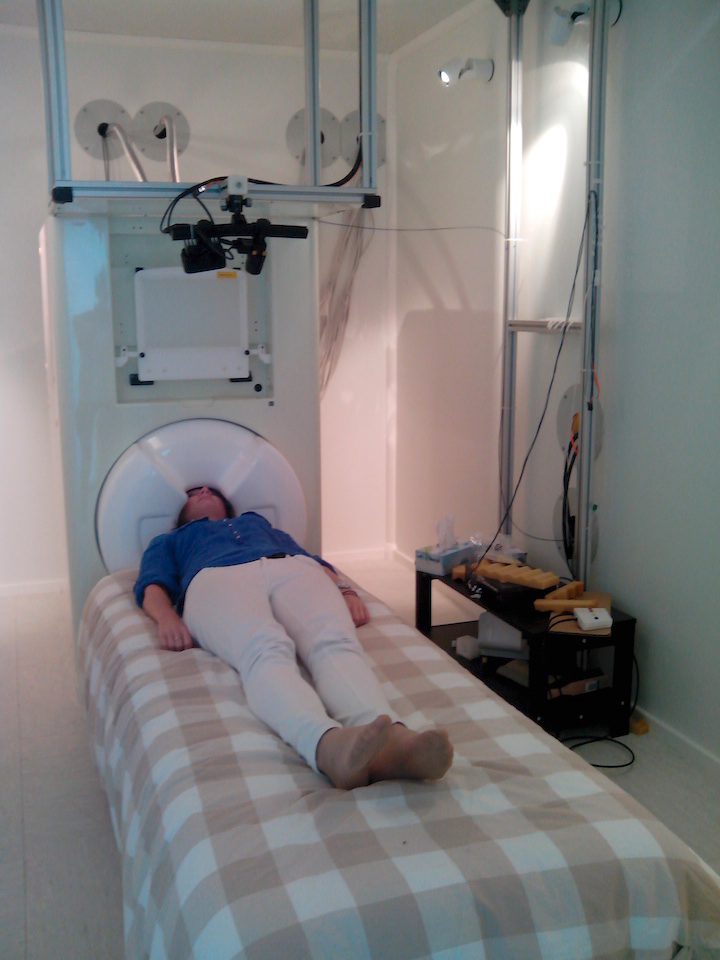
\includegraphics[height=0.95\textheight]{figs/meglab.png}\end{center}}

    \only<2->{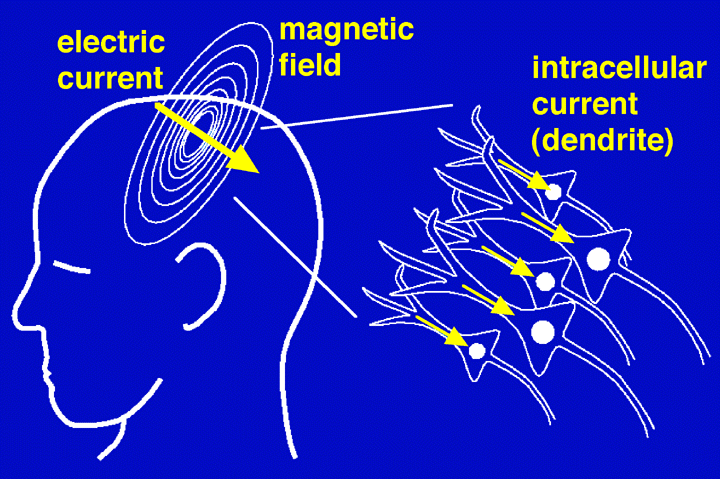
\includegraphics[scale=0.2]{figs/meg1.png}
	\hfill 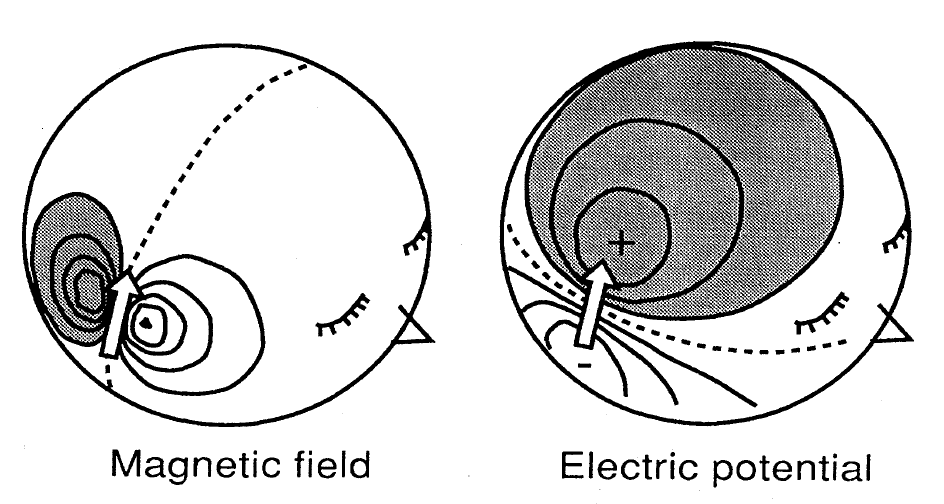
\includegraphics[scale=0.25]{figs/meg2.png}}

    \only<3->{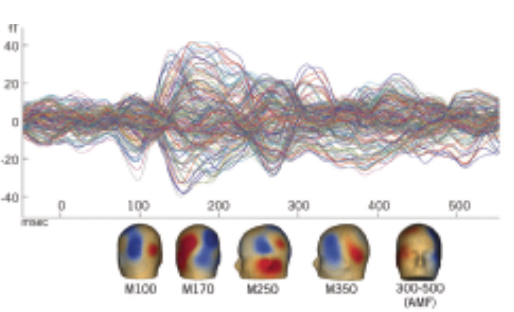
\includegraphics[scale=0.4]{figs/meg3.png}
	\hfill 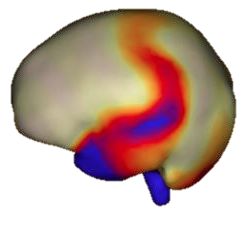
\includegraphics[scale=0.4]{figs/meg4.png}
    }
}

\frame{\frametitle{\insertsubsection: Priming in Irregular Verbs}
	\begin{block}{\cite{stockallmarantz06}}
		\begin{itemize} \tightlist
			\item Overt priming using \alert<1>{\textbf{MEG}}.
%			\bigskip
%			\item[] \includegraphics[scale=0.45]{figs/stockall1.png}
%			\bigskip
			
			\item[] 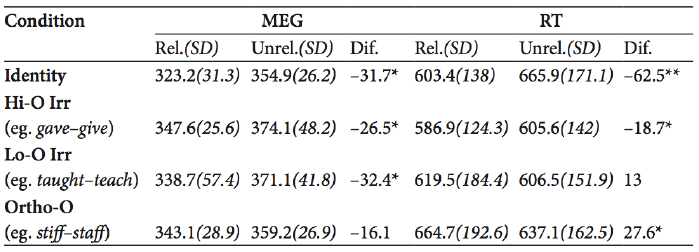
\includegraphics[scale=0.6]{figs/stockall2.png}
		\end{itemize}
%		\vspace{-0.5em}
		
	\end{block}
	
	\begin{itemize} \tightlist
		\item \alert<2>{\textbf{Finding:}} Priming for irregulars, including \emph{taught} priming TEACH.
		\item Their explanation: {[}\root{\gsc{TEACH}} + Past] primes \root{\gsc{TEACH}}.
	\end{itemize}
}


\frame{\frametitle{Interim Summary}
	\begin{enumerate}
		\item Suffixed nouns and adjectives are decomposed.
		\item Decomposition is obligatory.
		\item \alert{Irregular verbs are decomposed.}
		\item \alert{Can we predict how much?}
	\end{enumerate}
}


\frame{

	\large \centering
	
	Which stem is -\emph{able} more likely to appear after?
	
	\bigskip
	
	\emph{formidable} \hspace{3cm} \emph{taxable}
}


	\subsection{Transition probabilities}
\frame{\frametitle{\insertsubsection}

	\begin{itemize} \tightlist
		\item \emph{taxable}, \emph{taxing}, \emph{taxes}, \emph{taxation}, \dots{}
		\item \emph{formidable}, \dots{}?
	\end{itemize}

	\begin{block}{Transition probabilities}
		\begin{itemize} \tightlist
			\item \alert<2>{\textbf{Transition probability:}} the probability of having -\emph{able} after \emph{tax} or \emph{formid}.
			\item \emph{tax-able, formid-able}.
			\item Contrast with orthographic \emph{axab}, \emph{idab}.
		\end{itemize}
	\end{block}

	\begin{block}{M170}
		\begin{itemize} \tightlist
			\item Transition Probability: the \alert<3>{\textbf{probability}} of an affix given its stem.
			\item TP(formid\blue{able}) $>$ TP(tax\blue{able}).
			\item \alert<4>{\textbf{M170}}, a neural response originating at the fusiform gyrus, is sensitive to TP.
		\end{itemize}
	\end{block}
}


\frame{\frametitle{\insertsubsection: M170}
	
	\begin{block}{M170 effect (Solomyak and Marantz 2009)}
		\begin{itemize} \tightlist
			\item Materials: words suffixed with -\emph{able}, -\emph{ate}, \emph{ic}, \dots
			\item Transition probability modulates activation in the Visual Word Form Area.
			\item[] 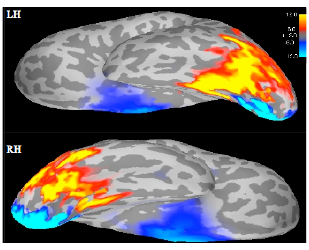
\includegraphics[height=0.3\textheight]{figs/solomyak1.png}
				\phantom{aaa}
			 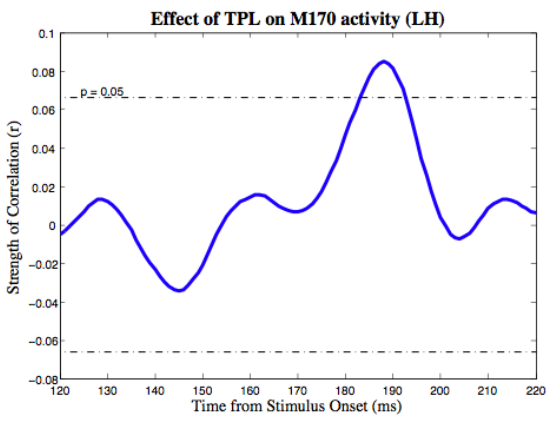
\includegraphics[height=0.3\textheight]{figs/solomyak2.png}
			\item Neural correlate of decomposition.
			\item TP(\emph{formidable} $>$ TP(\emph{taxable})
			\item M170(formid\blue{able}) $>$ M170(tax\blue{able}). \hfill \citey{\citep{solomyakmarantz10}}
		\end{itemize}
	\end{block}
	
	\ding{228} What about the \emph{brother} items?
}


\frame{\frametitle{\insertsubsection: M170}

	\begin{block}{Psuedo-affixes show M170 effects}
		\begin{itemize} \tightlist
			\item Even with pseudo-affixes. \hfill \citey{\citep{lewisetal11}}
			\item \emph{Broth\blue{er}}, \emph{lot\blue{ion}}, \emph{rat\blue{ion}}, \emph{mag\blue{ic}}, \emph{barb\blue{er}}, \emph{fin\blue{al}}, \dots
			\bigskip

			\item[] 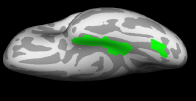
\includegraphics[height=0.26\textheight]{figs/lewis170roi.png} \phantom{aaa} 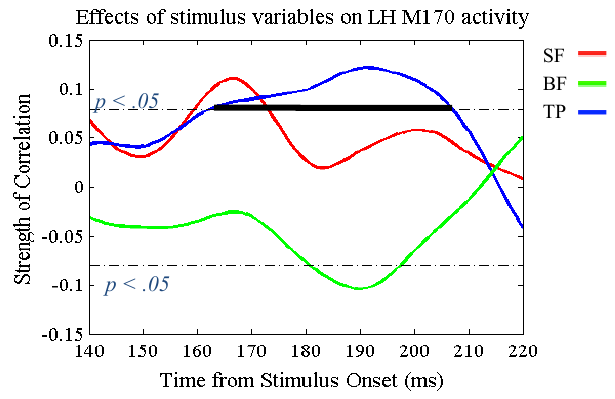
\includegraphics[height=0.26\textheight]{figs/lewis170res.png}
			\bigskip
			
%			\item[] 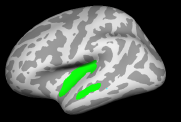
\includegraphics[height=0.3\textheight]{figs/lewis350roi.png} \phantom{aaa} 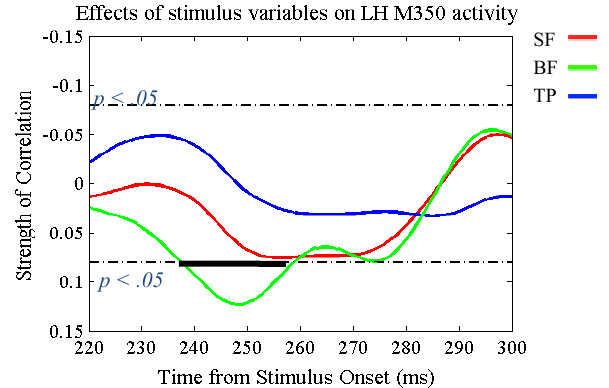
\includegraphics[height=0.3\textheight]{figs/lewis350res.png}
		\end{itemize}
	\end{block}
	
	\ding{228} Converging behavioral and MEG evidence for obligatory decomposition.
}


\frame{\frametitle{\insertsubsection: M170 and M350}

	We can even isolate different lexical statistic measures.
	
	\begin{block}{Lewis et al (2011)}
		\begin{itemize} \tightlist
			\item \emph{Lotion}, \emph{ration}, \emph{magic}, \emph{barber}, \emph{final}, \dots

			\item TP in M170: M170(formidable) $>$ M170(taxable)\\ 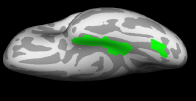
\includegraphics[height=0.26\textheight]{figs/lewis170roi.png} \phantom{aaa} 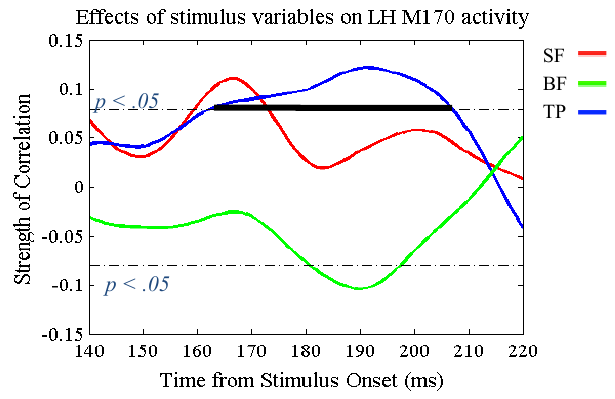
\includegraphics[height=0.26\textheight]{figs/lewis170res.png}
			
			\item Base frequency in M350: M350(taxable) $>$ M350(formidable)\\ 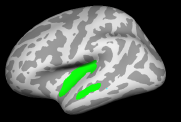
\includegraphics[height=0.3\textheight]{figs/lewis350roi.png} \phantom{aaa} 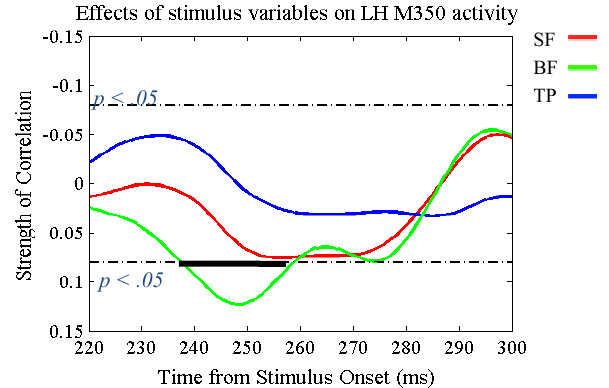
\includegraphics[height=0.3\textheight]{figs/lewis350res.png}
		\end{itemize}
	\end{block}
}


\frame{\frametitle{Regularity in Irregulars} \small

	Back now to irregular verbs:
	\begin{enumerate} \tightlist
		\item We have evidence that they are decomposed.
		\item We have measures for neural correlates of decomposition.
		\item We need measures for irregular verbs.
	\end{enumerate}
	
	\begin{block}{Albright and Hayes (2003)}
		\begin{itemize} \tightlist
			\item Past tense nonce words.
				\begin{itemize} \tightlist
					\item \emph{blafe}: \emph{blafed / bleft}?
					\item \emph{bredge: bredged / broge}?
					\item \emph{chake: chaked / chook}?
					\item \emph{fleep: fleeped / flept}?
				\end{itemize}
			\item[] 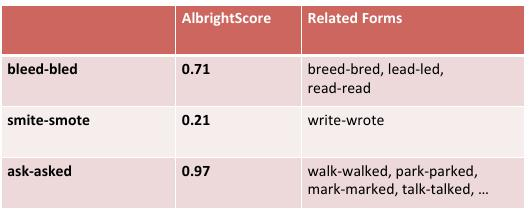
\includegraphics[scale=0.5]{figs/albrighthayes.jpg}
		\end{itemize}
	\end{block}
}



\frame{\frametitle{Tying it all together} \small
%	\begin{itemize}
%		\item[$\Rightarrow$] \alert<1>{\textbf{Working hypothesis:}} M170 is sensitive to identification of lexical items in the Visual Word Form Area. \hfill \citey{\citep{fruchtermarantz15,gwilliamsetal16tark}}.
%	\end{itemize}
	\alert<1>{\textbf{Return to irregular verbs:}} does \emph{taught} prime TEACH in masked priming?
	
	\cite{fruchteretal13}: \alert<2>{\textbf{yes}}. Priming found in M170 (and M350).
		\begin{center}
			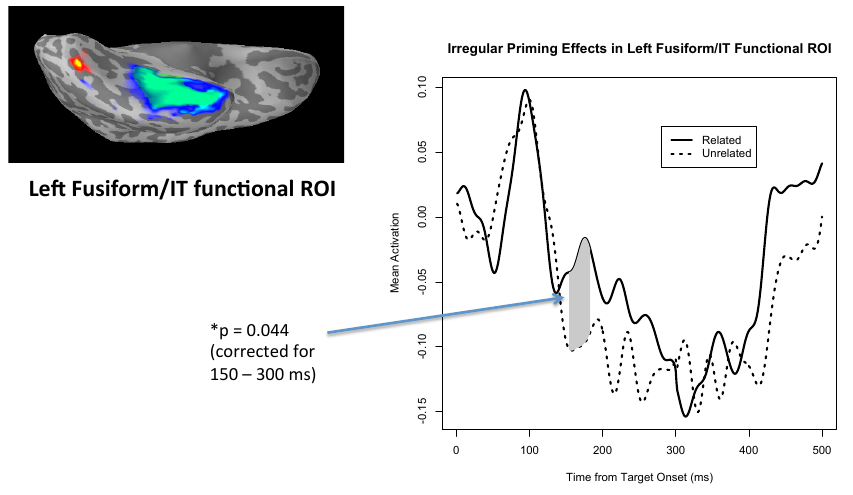
\includegraphics[scale=0.3]{figs/fruchter1.png}
		\end{center}
		
	\vspace{-2.1em}
		
	\alert<3>{\textbf{Correlated}} with strength of rule:
		\begin{center}
			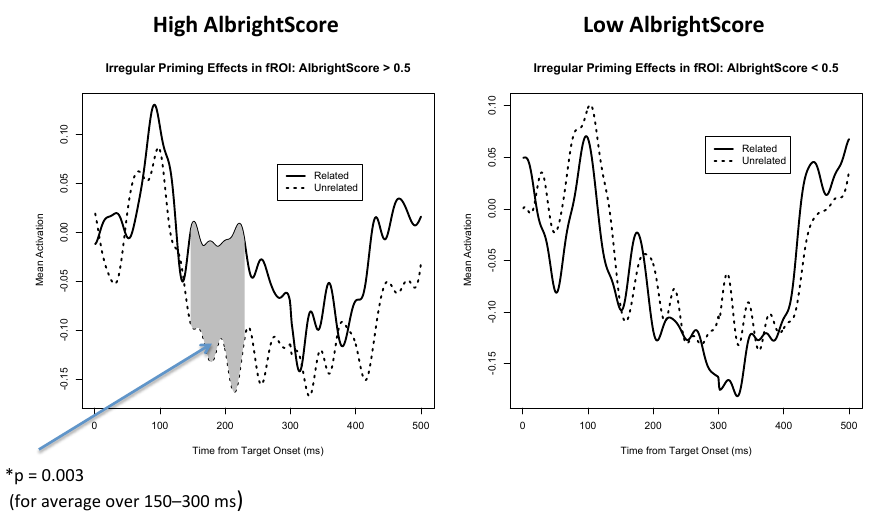
\includegraphics[scale=0.23]{figs/fruchter2.png}
		\end{center}
}

    \subsection{Infixation in Tagalog}
\frame{\frametitle{\insertsubsection}
    \begin{block}{Obligatory decomposition}
        \begin{enumerate}
            \item Complex forms (stem+affix) are decomposed.
            \item We seem to encode what affixes our language has.
            \item What if the affix is an infix?
        \end{enumerate}
    \end{block}

    Tagalog has prefixes, suffixes and infixes \citey{\citep{cayadoetal23}}:

    \begin{center}
        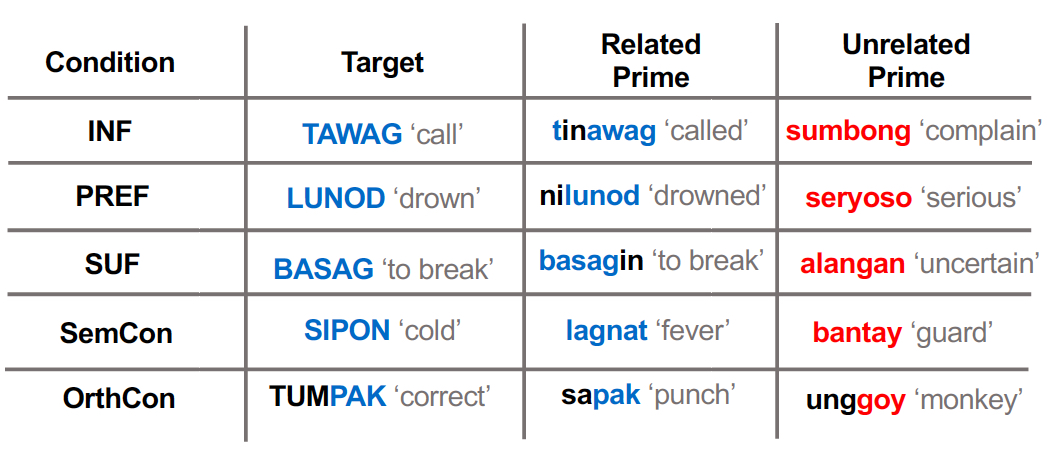
\includegraphics[width=0.8\textwidth]{figs/cayado1.jpg}
    \end{center}
}

    \subsection{Infixation in Tagalog}
\frame{\frametitle{\insertsubsection}

    % Tagalog has prefixes, suffixes and infixes \citey{\citep{cayadoetal23}}:

    % \begin{center}
    %     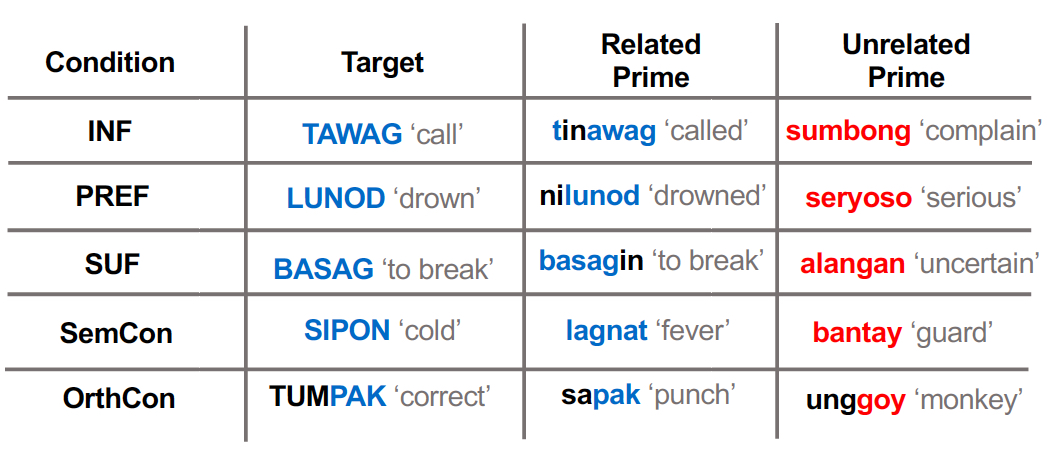
\includegraphics[width=0.4\textwidth]{figs/cayado1.jpg}
    % \end{center}

    \dots{} and all are decomposed in masked priming:
    
    \begin{center}
        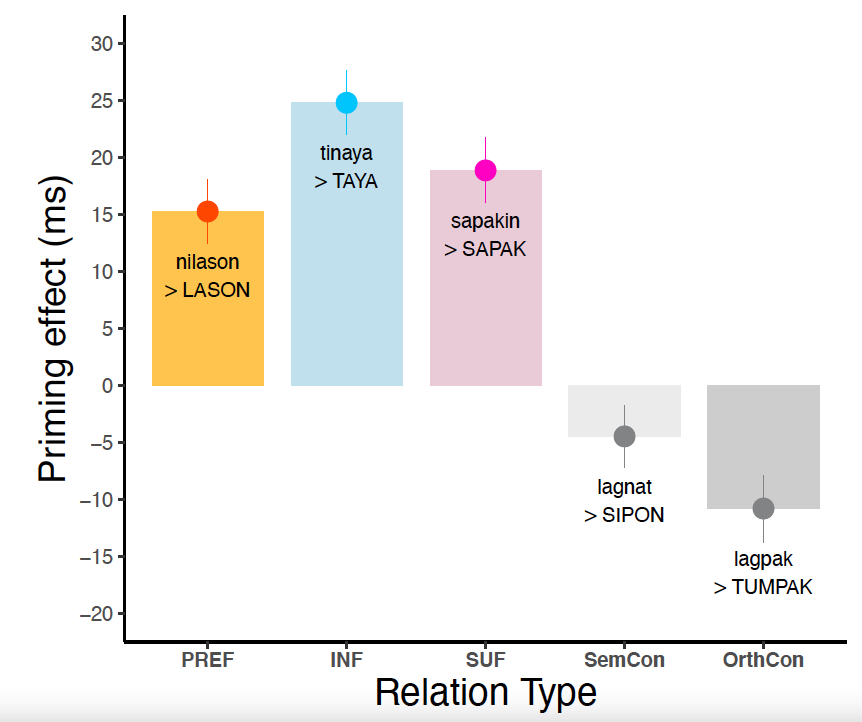
\includegraphics[width=0.75\textwidth]{figs/cayado2.jpg}
    \end{center}

    % \begin{center}
    % \begin{small}
    % \begin{tabular}{l|>{\em}l>{\em}ll|>{\em}l>{\em}ll}
    % \textbf{Condition} & \multicolumn{3}{c|}{\textbf{Related}} & \multicolumn{3}{c}{\textbf{Unrelated}} \\
    % Infix &  tinawag & TAWAG & called-TO CALL & sumbong & TAWAG & complain-TO CALL\\
    % Prefix & nilunod & LUNOD & drown-TO DROWN & seryoso & LUNOD & be serious-DROWN\\
    % Suffix & basagin & BASAG & get broken-TO BREAK & alangan & BASAG & be uncertain-TO BREAK\\
    % Semantic & lagnat & SIPON & fever-COLD & bantay & SIPON & guard-COLD\\
    % Orthographic & sapak & TUMPAK & punch-CORRECT & unggoy & TUMPAK & monkey-CORRECT\\
    % \end{tabular}
    % \end{small}
    % \end{center}
}

\frame{\frametitle{\insertsubsection}
    Tagalog infixation and pseudo-infixation \citey{\citep{wrayetal22}}: where should we get priming?

    \begin{center}
    \begin{tabular}{lllll}
    a.& \emph{subok} & `try' & \emph{sinubok} & `tried'\\
    b.& \emph{gulat} & `surprise' & \emph{ginulat} & `shocked someone'\\
    c.& *\emph{noŋ} & --- & \emph{ninoŋ} & `godfather'\\
    d.& *\emph{mistro} & --- & \emph{ministro} & `ministry'\\
    \end{tabular}
    \end{center}
    
\bigskip

    \only<2>{
    \begin{center}
    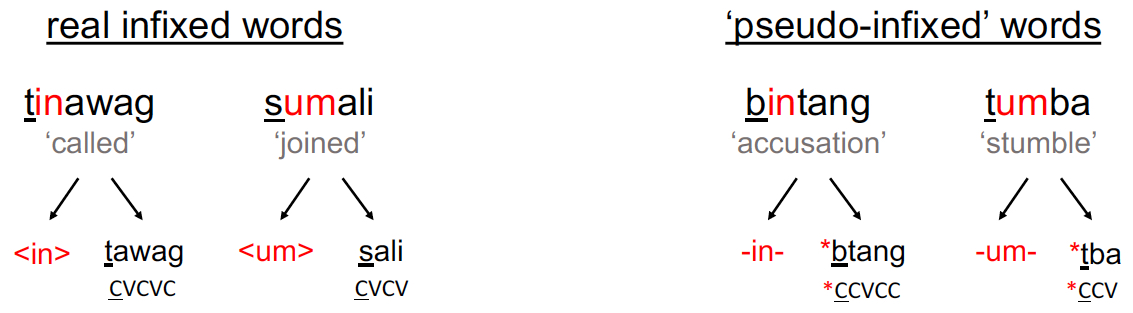
\includegraphics[width=0.9\textwidth]{figs/tagalog.jpg}
    \end{center}
    
\bigskip

    \ding{228} See \cite{wrayetal22} for discussion of the M170 in Tagalog infixes, pseudo-infixes and reduplication.    
    }
}


	\subsection{Nonconcatenative morphology}
\frame{\frametitle{\insertsubsection}

	We've seen converging evidence that morphologically complex forms are decomposed into constituent morphemes.
	\bigskip

	There's a wealth of work on processing Semitic.\\
\citey{\citep{frostetal97,frostetal00jeplmc,deutschetal98,deutschetal00,deutschetal03,deutschetal05,deutschmeir11,velanetal05,bicketal08,bicketal10,boudelaamarslenwilson05,boudelaamarslenwilson11,boudelaaetal10,twist06,ussishkintwist09,ussishkinetal11,schluter13,ussishkinetal15,fmdpmetal05jml,gwilliamsmarantz15,farhyetal17}}
		
	\bigskip
	
	Main findings: robust root priming and some template priming.
	
	\bigskip
		
	What does this look like? How abstract can the representation of these morphemes be? 
}


\frame{\frametitle{\insertsubsection}
	\vspace{-0.5em}
	
	\begin{small}
	Work by Deutsch, Frost and colleagues:
	\end{small}
	\vspace{-0.5em}
	
	\begin{center}
	\begin{tabular}{lllcl}
%		\cmark & \textbf{Root priming:} & \emph{\textbf{z}a\textbf{m}a\textbf{r}} & --- & \emph{TI\textbf{ZM}O\textbf{R}ET}\\
%			&			&	 { זמר} & & { תזמורת} \\
%			&			&	`singer' & & `band'\\
		
		\cmark & \alert<1>{\textbf{Root priming:}} & \alert<1>{\textbf{לבש}}{הת} & --- & {\Large \alert<1>{\textbf{ש}}{י}\alert<1>{\textbf{לב}}{ה}}\\
			&			&    \emph{hit\alert<1>{\textbf{l}}a\alert<1>{\textbf{b}}e\alert<1>{\textbf{ʃ}}} & & \emph{he\alert<1>{\textbf{lb}}i\alert<1>{\textbf{ʃ}}} \\ 
			&			&  `got dressed' & & `dressed someone up'\\
			
		\cmark & \alert<2>{\textbf{Template priming:}} & {ט}\alert<2>{\textbf{י}}{סר}{\alert<2>{\textbf{ה}}} & --- & {\Large {ק}\alert<2>{\textbf{י}}{ספ}{\alert<2>{\textbf{ה}}}}\\ 
			&			&  \emph{\alert<2>{\textbf{he}}sr\alert<2>{\textbf{i}}t} & & \emph{\alert<2>{\textbf{he}}sp\alert<2>{\textbf{i}}k}\\
			&			&  `filmed' & & `sufficed'\\\hdashline
			
		\xmark & \alert<3>{\textbf{Pattern priming:}} & {ט}\alert<3>{\textbf{י}}{קל}\alert<3>{\textbf{ת}} & --- & {\Large {ל}\alert<3>{\textbf{י}}{רג}\alert<3>{\textbf{ת}}}\\
			&			& \emph{\alert<3>{\textbf{ta}}kl\alert<3>{\textbf{i}}t} &  & \emph{\alert<3>{\textbf{TA}}RG\alert<3>{\textbf{I}}L}\\
			&			& `record' & & `exercise'\\\hdashline

		
		\textbf{?} & \alert<4>{\textbf{Abstract template}} & {צלל} & --- & {\Large רחץ}\\
			&			& \emph{\texttslig alal} &  & \emph{raxa\texttslig}\\
			&			& `dove'  &  & `washed'\\		
	\end{tabular}
	\end{center}
	\vspace{-0.5em}
	
	Three characters aren't enough to \alert<5>{\textbf{identify the verb/template}}:
	\begin{enumerate}
		\item basar { בשר}
		\item halax { הלך}
		\item katan { קטן}
	\end{enumerate}
}


\frame{\frametitle{\insertsection}
	\alert<1>{\textbf{What we know:}}
	\begin{enumerate} \tightlist
		\item Affixes are obligatorily decomposed.
		\item M170 tracks decomposition.
		\item Roots are primed.
		\item Templates are primed (sometimes).
	\end{enumerate}
	
	\begin{block}{\alert<2>{\textbf{Hypotheses}}}
		\begin{itemize} \tightlist
			\item[A] Visual word decomposition only tracks overt forms/morphemes.
			\item[B] Visual word decomposition tracks abstract morphemes as well.
		\end{itemize}
	\end{block}
	
	\begin{block}{\alert<3>{\textbf{Methods}} \citey{\citep{kastneretal18}}}
		\begin{itemize} \tightlist
			\item Visual lexical decision using MEG.
			\item Masked priming, SOA = 33ms.
			\item N = 21 native speakers of Hebrew.
			\item 42 verbal targets in {\tkal}, matched with primes.
		\end{itemize}
	\end{block}
}

		
\frame{\frametitle{\insertsection}  \small
	\begin{block}{Materials}
		\begin{center}
%		\begin{small}
		\begin{tabular}{|l|lll|lll|} \hline
						& \multicolumn{3}{c|}{\textbf{Shared \blue{Template}}}		& \multicolumn{3}{c|}{\textbf{Shared \red{Root}}}\\
						& Ortho & Phono & Gloss			& Ortho & Phono & Gloss \\\hline
		\textbf{Related} 	&  {צלל} & {\texttslig}\blue{a}l\blue{a}l & `dove' 						& {התרחץ}				& hit\red{r}a\red{x}e\red{\texttslig}	& `washed himself'\\	
		\textbf{Unrelated} & {בשר} & basar 				& `meat'						& {התלבש}				& hitlabeʃ & `dressed up'\\\hline\hline
		\textbf{Target}		& \multicolumn{2}{c}{ רחץ} & \multicolumn{2}{c}{\red{r}\blue{a}\red{x}\blue{a}\red{\texttslig}} & \multicolumn{2}{c|}{washed (transitive)} \\\hline
		\end{tabular}
%		\end{small}
		\end{center}

		\begin{itemize}
			\item All strings were unambiguous.
			\item Unrelated Shared Template prime (`meat'): adjectives and nouns.
			\item Ssyntactic category cannot be known from the orthography or phonology alone.
		\end{itemize}
	\end{block}
}



\frame{\frametitle{\insertsection} 
	\begin{block}{Results}
 	\begin{columns}
 		\begin{column}[b]{0.5\textwidth}
	 		\begin{center}\textbf{\blue{Shared template}}\end{center}
			\begin{itemize} \tightlist
				\item Significant effect of Relatedness.
				\item $p<0.01$.
				\item 177-219ms.
				\item \alert<1>{\textbf{Novel result:}} verbs in {\tkal} prime other verbs in {\tkal}.
			\end{itemize}
		\end{column}
		\begin{column}[b]{0.4\textwidth}
			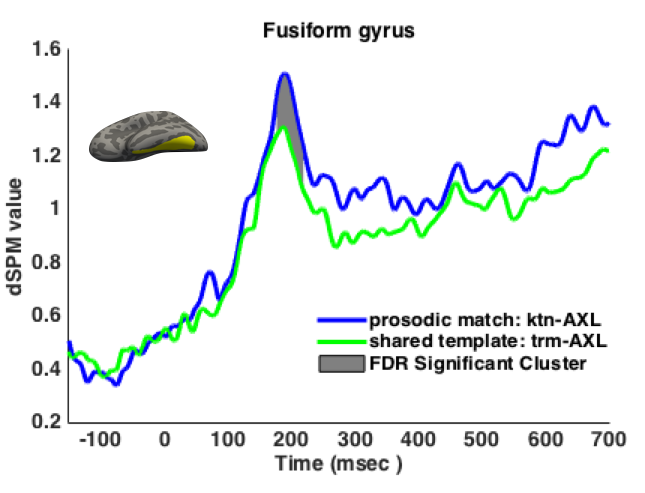
\includegraphics[width=1\textwidth]{figs/ff170.png}
		\end{column}
	\end{columns}
	\end{block}
		
	\begin{enumerate}
		\item Replicated findings for root and template priming in {\thif} (not shown).
		\item No root priming in this template, as noted in the behavioral literature before (remains mysterious).
	\end{enumerate}
}


\begin{frame}[noframenumbering] \footnotesize %,allowframebreaks]		
	\frametitle{Full experimental design}
	\begin{columns}[t]
		\begin{column}{0.5\textwidth} \centering
			Experiment 1: {\thif}
			
			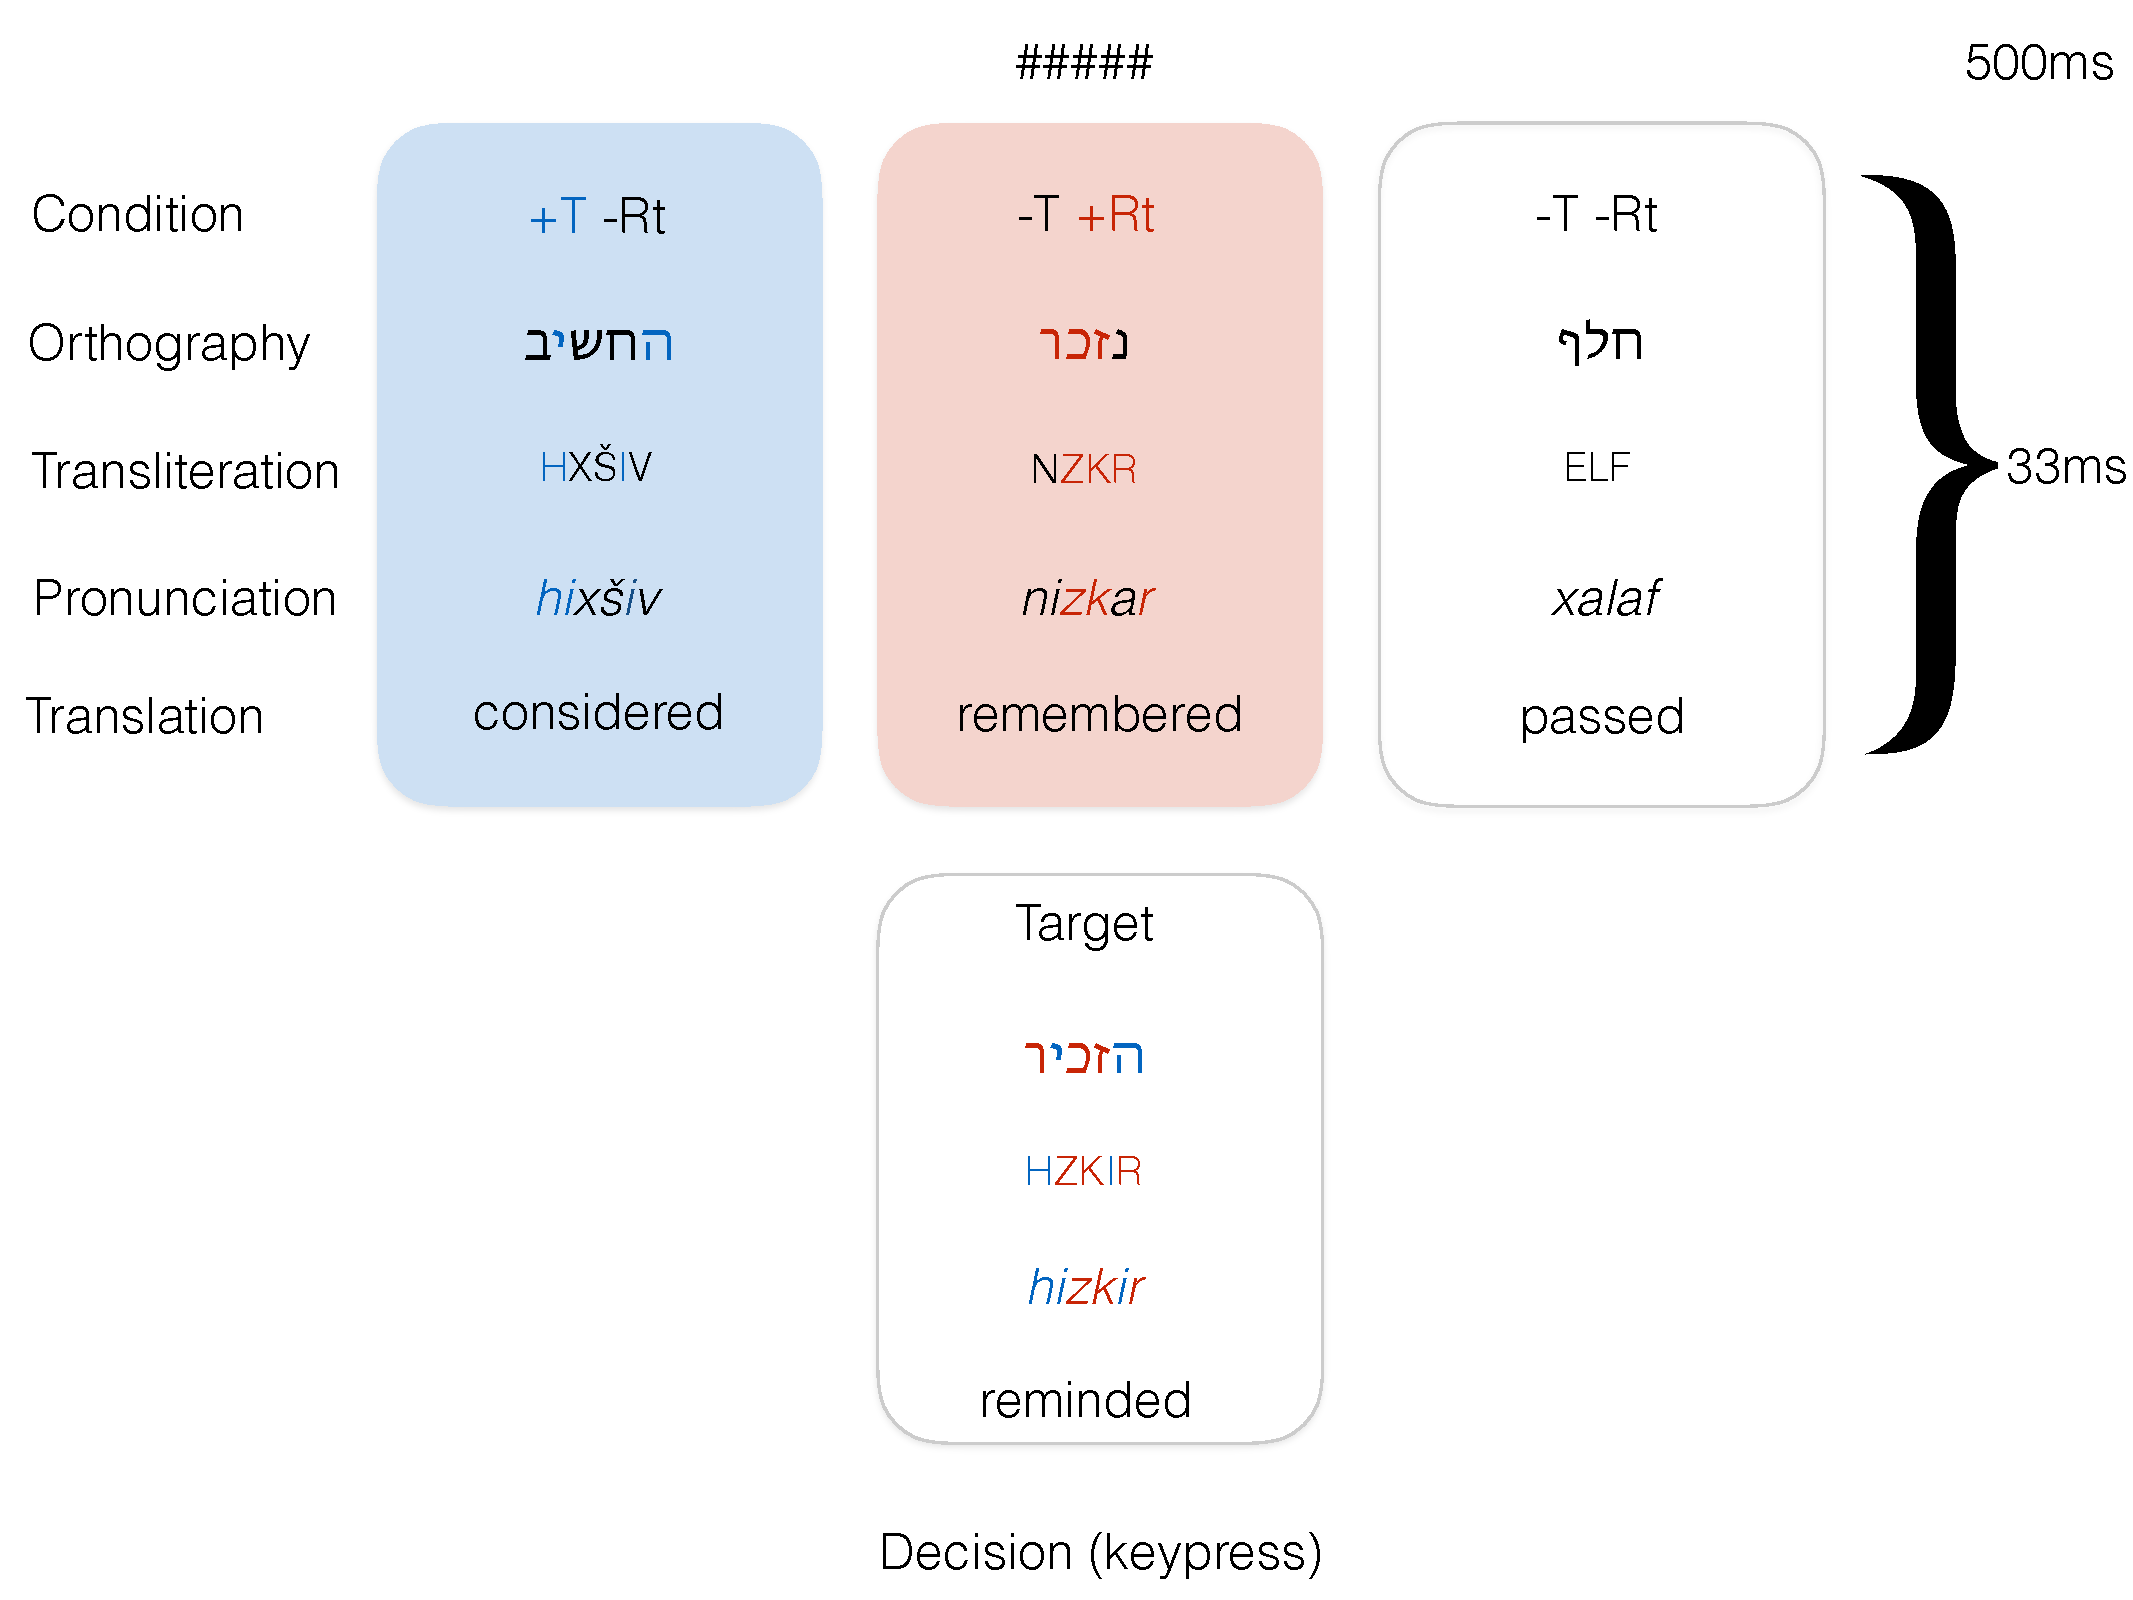
\includegraphics[width=0.8\textwidth]{figs/fig2.pdf}
			\vfill
			
			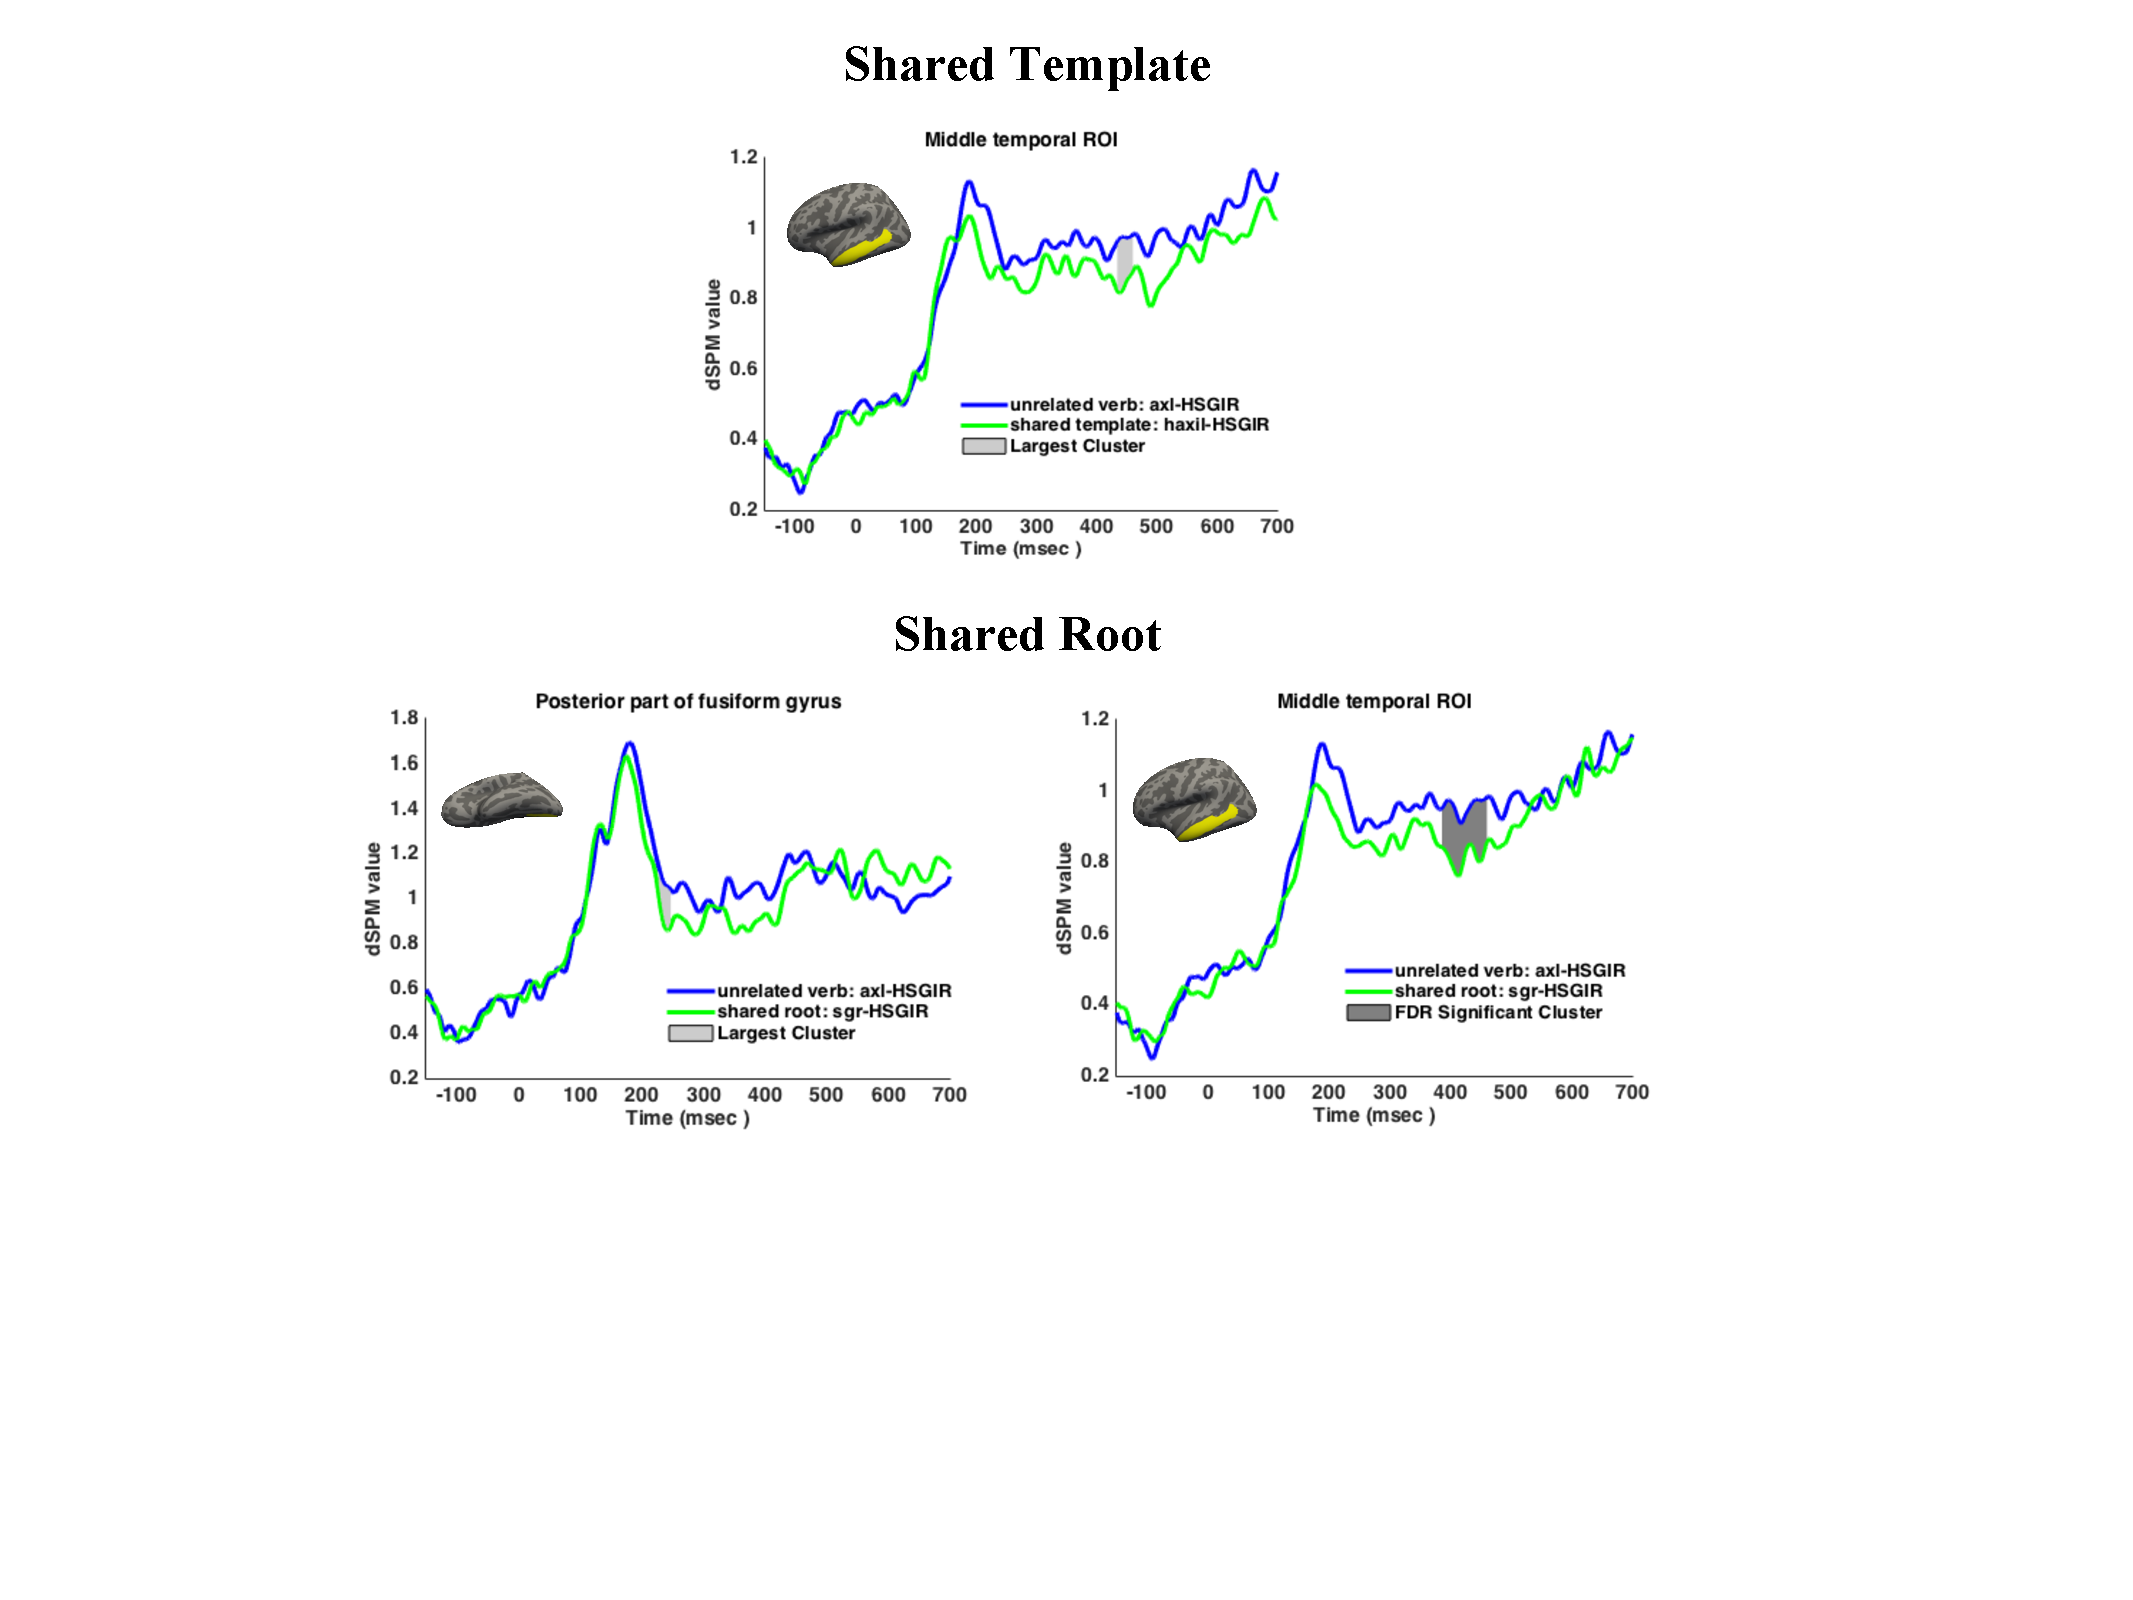
\includegraphics[width=0.8\textwidth]{figs/fig4.pdf}		
		\end{column}
		\begin{column}{0.5\textwidth} \centering
			Experiment 2: {\tkal}
			
			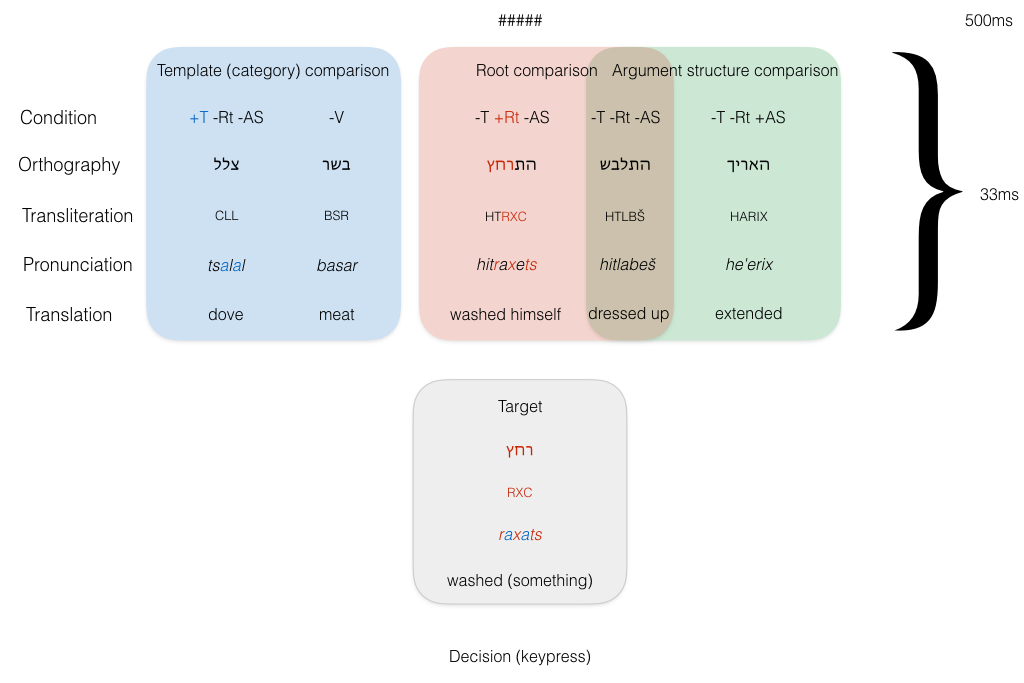
\includegraphics[width=0.8\textwidth]{figs/fig5.001.jpeg}
			\bigskip
			
			\vfill
			
			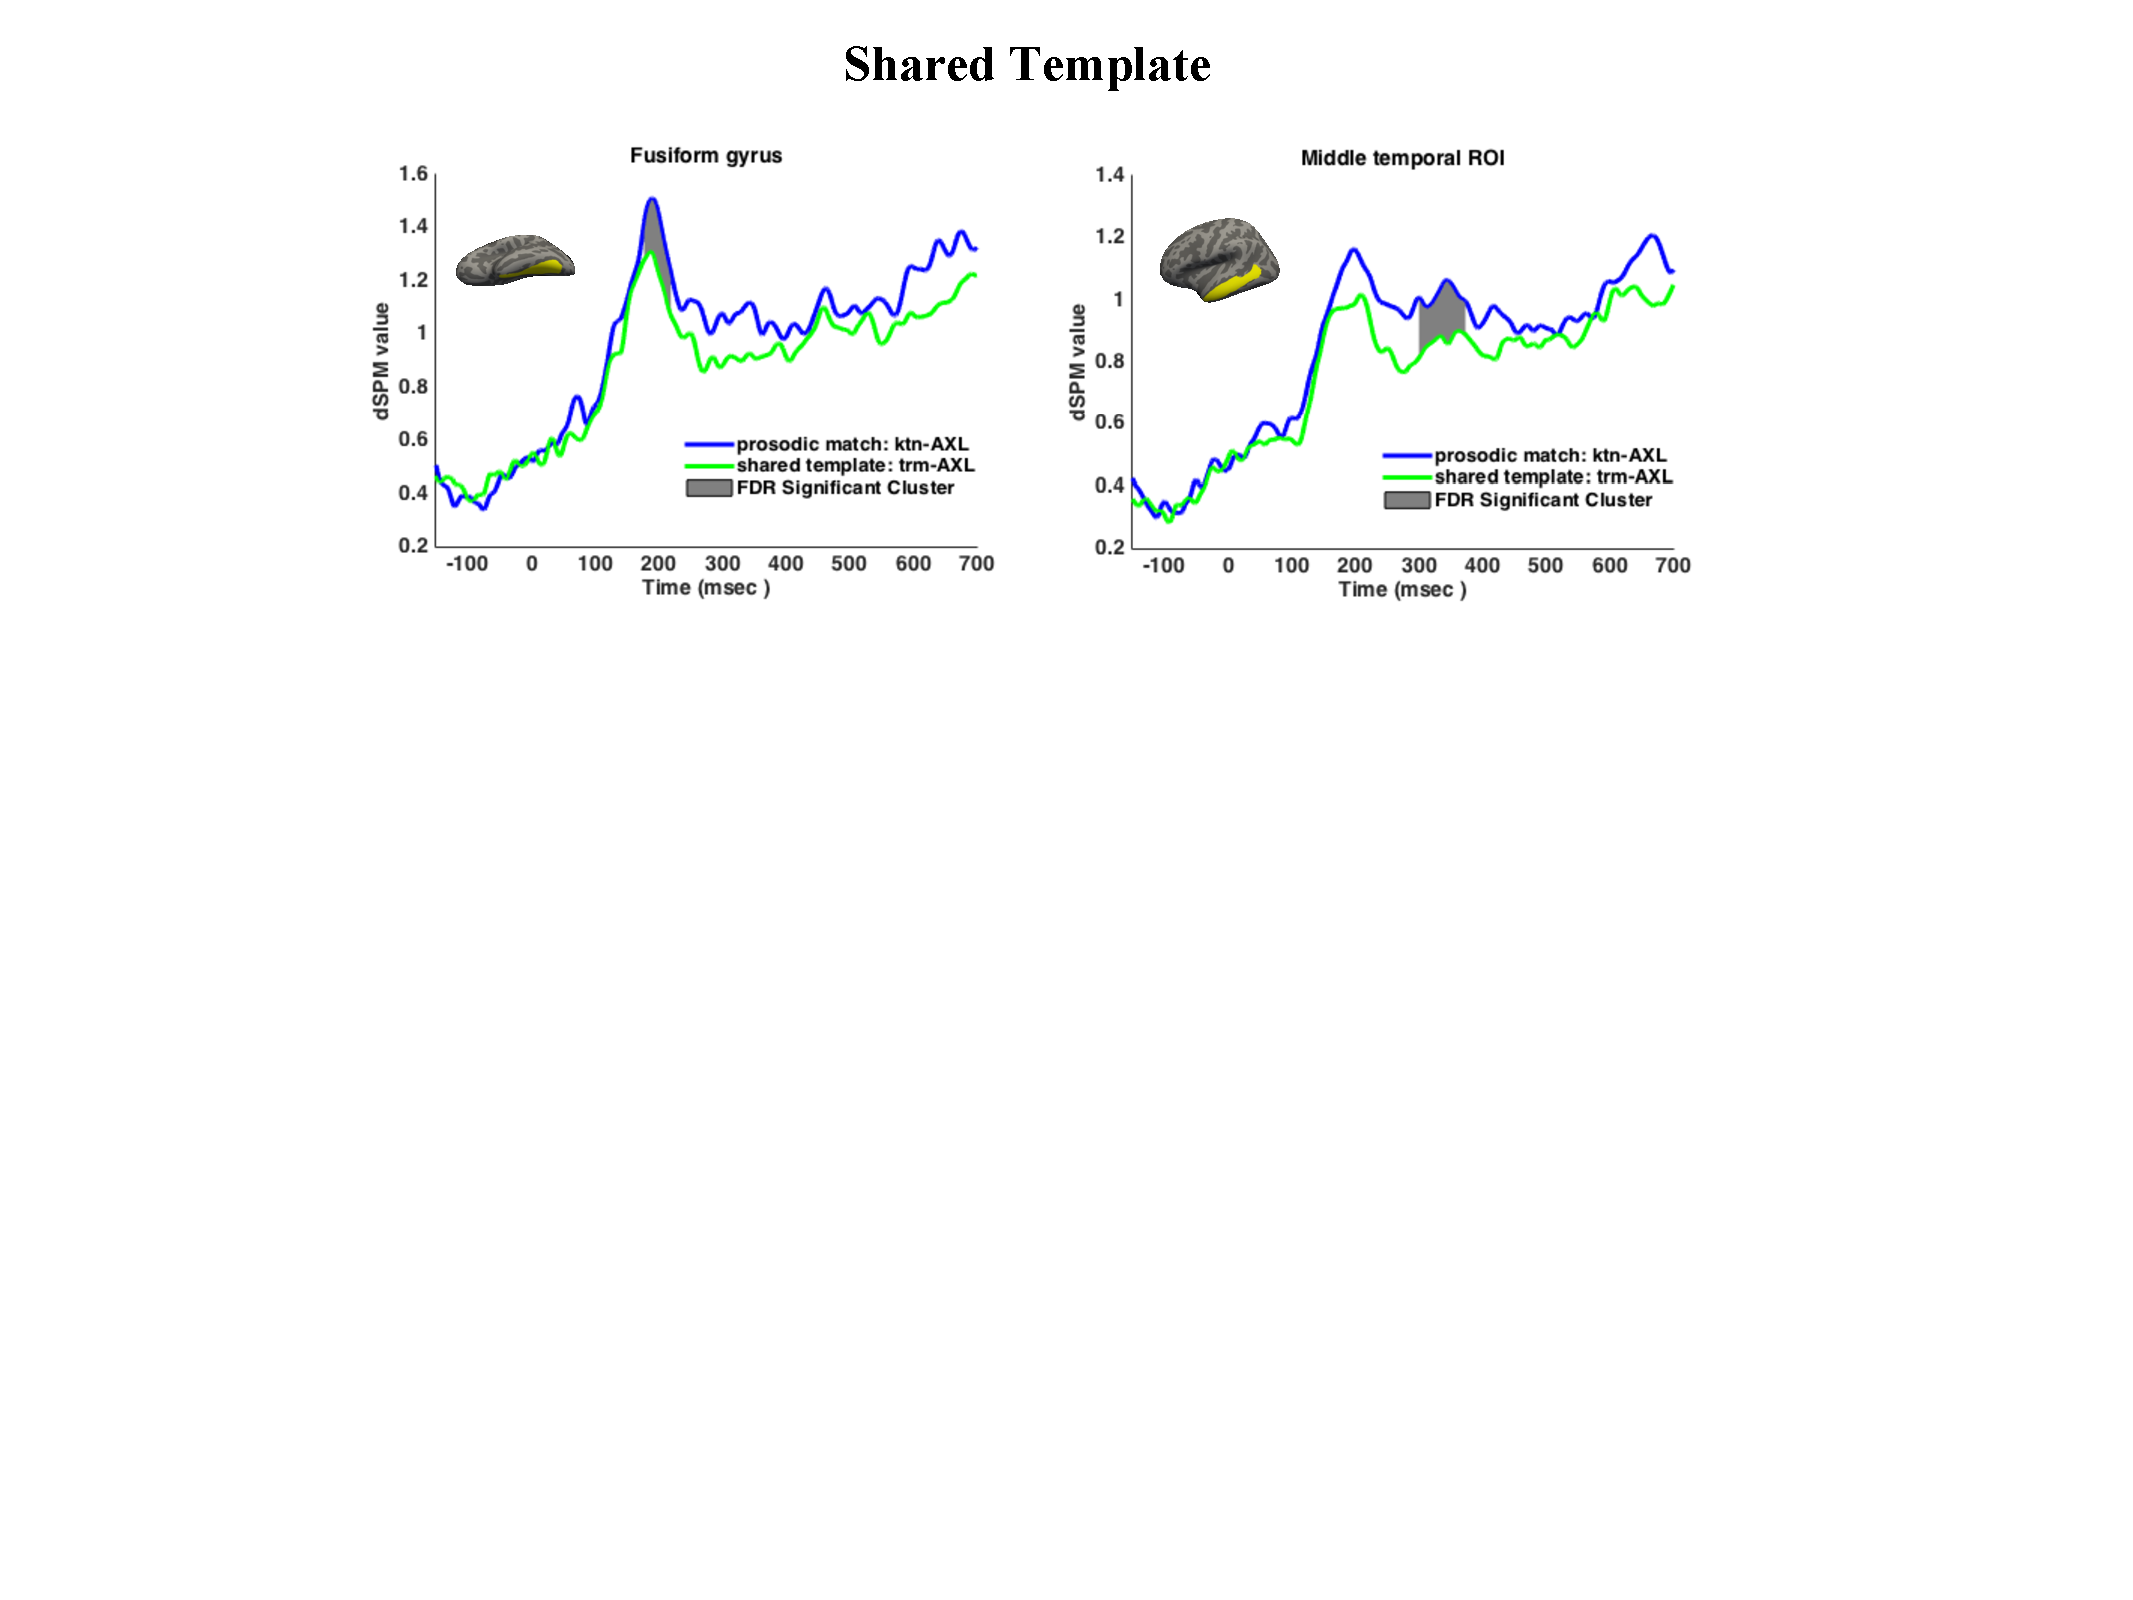
\includegraphics[width=0.8\textwidth]{figs/fig6.pdf}		
		\end{column}
	\end{columns}
\end{frame}


\frame{\frametitle{\insertsubsection}
	\begin{block}{Discussion}
		\alert<1>{\textbf{Implications:}}
		\begin{itemize} \tightlist
			\item If a Hebrew string XYZ can be immediately parsed into [\root{XYZ} v], it is.
			\item Abstract v may then be primed again, even if it is covert.
			\item[$\Rightarrow$] Support for Hypothesis B: readers recognize abstract morphemes too.
		\end{itemize}
		
		\alert<2>{\textbf{In general:}}
		\begin{itemize} \tightlist
			\item In line with the literature on form-based masked priming.
			\item Provides an explanation for masked priming results beyond matching of overt forms.
			\item[$\Rightarrow$] Beyond ``priming morphemes'': experimental findings only make sense given a theory of the task (a linking theory).
		\end{itemize}
	\end{block}
}


\begin{frame}{Additional references}
	\begin{itemize}
		\item Work in this general approach:
			\begin{itemize}
			\item Prefix/particle priming: \cite{creemersetal20jml}
			\item Plural affix priming: \cite{goodwindaviesembick19}
			\item Auditory priming: \cite{schluter13,ussishkinetal15}
			\item Rhyme auditory priming: \cite{bacovcinetal17}
			\item Argument structure: \cite{gwilliamsmarantz18,neophytouetal18}
			\item Nouns vs verbs: \cite{kingetal14}
            \item Insights from Tagalog (e.g.~reduplication): \cite{cayadoetal23}
			\end{itemize}
		\item One alternative view: \cite{baayenetal11,baayenetal15lcn,marantz13lcp}
		\item Word processing in a syntactic context: \cite{lukechristianson11}
		\item Overviews: \cite{crepaldi23taf,stockallgwilliams20cup}
	\end{itemize}
\end{frame}


\frame{\frametitle{Goals, revisited}
\begin{itemize}
	\item Discuss	 one major	 issue of	 morphology	 in	 the	  psycholinguistic	 and neurolinguistic	literature.	
  
	\item Most studies	 ask	 whether	 words	 decompose	 into	morphemes	 during	 language	 recognition	 and	 production.
  
	\item Some	 hypotheses	 suggest	 that	 decomposition	 varies	  depending	 on	 the	 ``transparency'' or	 ``regularity'' of	 the	morphology.
  
  \item   We	 looked	 at	 evidence	 that	 words	 are	  decomposed	 no	 matter	 how	 ``opaque'' and	 ``irregular''.
  
  \item Even when the morphemes are abstract, e.g.~a verbalizer in Hebrew.
\end{itemize}
}


\appendix
\begin{frame}[noframenumbering,allowframebreaks]
	\frametitle{References}
%	\scriptsize
	\tiny
	\bibliographystyle{linquiry2}
	\bibliography{lingxbib}
\end{frame}



\end{document}

\begin{columns}[t]
	\begin{column}{0.5\textwidth}
	\end{column}
	\begin{column}{0.5\textwidth}		
	\end{column}
\end{columns}